\documentclass[11pt]{article}
\usepackage{tikz}
\usetikzlibrary{trees}
\usepackage{forest}
\usepackage{hyperref}
\usepackage{multirow}
\usepackage{graphicx}
\usepackage{amsmath}

%Gummi|065|=)
\title{\textbf{Shannon Entropy from Data Compression Perspective}}
\author{K{\i}van\c{c} \c{C}akmak\\}
\date{}
\begin{document}

\maketitle

In this article, I'll try to explain Shannon Entropy with one of its use case: data-compression. First, I'll provide a small introduction about data-representation and a need for compression with very brief information about its requirements. Consequently, I'll derive the proof of well-known entropy formula in the equation below that estimates the average minimum number of bits needed to encode information with priorly known probabilities:

\begin{equation}
H(X) = -\sum_{i}p_{i}\log_{b}p_{i}
\label{Eq:entropy}
\end{equation}

\section{Data Representation and Compression}

We all know that the way that our digital devices store data as ones and zeros, aka in binary format. So, our understanding of the smallest chunk of information is: "whether there is a voltage or not". 
We represent letters of a text, pixels of an image, etc. in binary format. 

Below, I provide an ASCII (American Standard Code for Information Interchange) encoded \textit{hello} in Table \ref{table:hello}. In ASCII, each letter -and other control characters, such as \texttt{DEL} and numbers like $1$, $2$ etc.- consists $8$ bits. So, the text that we see is \texttt{hello}, but the information that a digital device stores are: 
\begin{center}
    \texttt{0110100001100101011011000110110001101111}
\end{center}

\begin{figure}
\begin{tabular}{| l | l | l | l | l | l |}
 \hline
  text   & h & e & l & l & o\\ \hline
  ASCII  & 104 & 101 & 108 & 108 & 111 \\ \hline 
  binary & 01101000 & 01100101 & 01101100 & 01101100 & 01101111 \\ 
  \hline
\end{tabular}
\caption{ASCII encoding of \textit{hello}.}
\label{table:hello}
\end{figure}

So, there are $26$ letters in the English alphabet, and we can say that $5$ bits would be enough to encode all characters, since $2^{5} = 32 > 26$. Nevertheless, ASCII has 127 different values --See Reference \cite{ascii}, which at least requires 7 bits per value. 

The rest of the document tries to answer the following question:

\begin{center}
\textit{What would be the minimum number of bits that we have to use if we knew the distribution of letters for a particular text that we have?}
\end{center}

\begin{figure}[ht!]
\centering
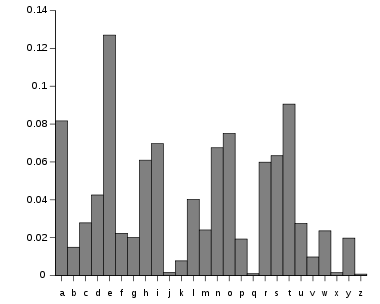
\includegraphics[width=\linewidth]{img/english_histogram.png}
\caption{Frequency Table of English Letters \label{fig:letter_histogram}}
\end{figure}

So, as it could be seen in Figure \ref{fig:letter_histogram} --and we all very well know, some of the letters are more often used than the others. Here, \textit{e} is the most commonly used letter in English. So, would it be better to represent \textit{e} with fewer bits than the others, if the letter distribution of our text would be exactly the same with Figure \ref{fig:letter_histogram}. If so, how less could it be?

\section{Uniquely Decodable Codes}
A code is a mapping of \textit{source messages} into \textit{codewords}. As an example, ASCII code above maps letters (as a source message) to codewords --such as \textit{h} to 01101000. 

Here, a code is \textit{distinct} if each codeword is distinguishable from every other (i.e., the mapping from source messages to codewords is one-to-one). A distinct code is \textit{uniquely decodable} if every codeword is identifiable in a sequence of codewords. 

\subsection{Prefix Codes}
A uniquely decodable code is called a \textit{prefix code} (or prefix-free code) if it has the prefix property, which requires that no codeword is a proper prefix of any other codeword.

\begin{figure}[h!]
\begin{center}
\begin{tabular}{| l | l | l | l | l |}
 \hline
  text   & a & b & c & d \\ \hline
  binary & 0 & 01 & 011 & 0111 \\ 
  \hline
\end{tabular}
\caption{Uniquely decodable non-prefix code}
\label{table:non_prefix_code}
\end{center}
\end{figure}

The code in Figure \ref{table:non_prefix_code} is decodable but it is not a prefix code because the codeword for \textit{a} is a prefix for the codeword for \textit{b}. This means that we can not instantaneously decode \textit{a} without waiting for the next bit of data (to determine whether it is actually \textit{a} or just the first half of \textit{b}.)

\begin{figure}[h!]
\begin{center}
\begin{tabular}{| l | l | l | l | l |}
 \hline
  text   & a & b & c & d \\ \hline
  binary & 0 & 111 & 1011 & 1010 \\ 
  \hline
\end{tabular}
\caption{Uniquely decodable prefix code}
\label{table:prefix_code}
\end{center}
\end{figure}

Alternatively, the code in Figure \ref{table:prefix_code} is a prefix code, since no codeword is a prefix of another codeword.

\section{Kraft's Inequality}

Kraft's inequality states that given a list of positive integers ($n_{1}, n_{2}, \dots, n_{r}$), there exists a prefix code with a set of codewords ($\sigma_{1}, \sigma_{2}, \dots, \sigma_{r}$) where the length of each codeword $|\sigma_{i}| = n_{i}$, $\forall_{i}$, if and only if:

\begin{equation}
\sum_{i=1}^{r} s^{-n_{i}} \leq 1
\end{equation}

where \textit{s} is the size of the alphabet \textit{S}.

Our previous example code in Figure \ref{table:prefix_code}, the alphabet is simply the binary digits $S = {0, 1}$, and therefore the size of the alphabet $s = 2$. We can easily check that indeed the inequality holds:

\begin{equation}
2^{-1} + 2^{-3} + 2^{-4} + 2^{-4} \leq 1
\end{equation}

\subsection{Proof}

As it could be observed in Figure \ref{fig:kraft_tree}, there are $s^{n_{j}}$ combination of codewords where we could chose for $j_{th}$ level if there was no prefix constraints, but due to the codeword at a prior level $k < j$, $s^{n_{j} - n_{k}}$ amount of codewords are forbidden, since they contain $\sigma_{k}$ as a prefix. 

In other words, to satisfy prefix-code requirements, each codeword must be represented by a leaf node, since it has to eliminate its descendants as codewords.

\begin{center}
\begin{figure}[h!]
\begin{center}
\begin{forest}
for tree={circle,draw, l sep=1cm, s sep=0.6cm, minimum height=1cm, minimum width=1cm}
[, 
    [1,edge label={node[midway,left] {$2^{-1}$}}
        [11,edge label={node[midway,left] {$2^{-2}$}}
            [111,edge label={node[midway,left] {$2^{-3}$}}]
            [110,edge label={node[midway,right] {$2^{-3}$}}]
        ] 
        [10,edge label={node[midway,right] {$2^{-2}$}}
            [101,edge label={node[midway,left] {$2^{-3}$}}]
            [100,edge label={node[midway,right] {$2^{-3}$}}]
        ] 
    ]
    [0,edge label={node[midway,right] {$2^{-1}$}}
        [01,edge label={node[midway,left] {$2^{-2}$}}
            [011,edge label={node[midway,left] {$2^{-3}$}}]
            [010,edge label={node[midway,right] {$2^{-3}$}}]
        ] 
        [00,edge label={node[midway,right] {$2^{-2}$}}
            [001,edge label={node[midway,left] {$2^{-3}$}}]
            [000,edge label={node[midway,right] {$2^{-3}$}}]
        ] 
    ] 
]
\end{forest}
\end{center}
\caption{Code Tree}
\label{fig:kraft_tree}
\end{figure}
\end{center}

So, a codeword at level $j$ has $s^{n_{r}-n_{j}}$ descendants (where $n_{r}$ is the length of longest codeword) at the highest level. For instance $1$ has $2^{3-1}$ descendants which are $111$, $110$, $101$ and $100$.

Besides, descendant sets of codewords must be disjoint to satisfy prefix-free requirement. As an example, $1$ and $10$ has joint descendants, which are $101$ and $100$, hence a prefix-free codeword can not contain $1$ and $10$.

So, we know that the total number of forbidden codewords at step $j$ is:

\begin{equation} \label{eq1}
\sum_{i=1}^{j-1} s^{n_j - n_i} \\
\end{equation}

As an example, if our level $j=3$, we would have 6 forbidden codewords which can also be observed from the Code Tree in Figure \ref{fig:kraft_tree}:

\begin{equation} \label{eq1}
\begin{split}
\sum_{i=1}^{j-1} s^{n_j - n_i} = 2^{(3-1)} + 2^{(3-2)} = 6
\end{split}
\end{equation}

For each level $j$, we possibly have $s^{n_j}$ codewords; and this amount should exceed the number of forbidden codewords for level $j$ to have a prefix codeword set. Here we apply this lemma for highest level $r$ below, which implies the Kraft Inequality:

\begin{equation} \label{eq1}
\begin{split}
\sum_{i=1}^r s^{n_r - n_i} \leq s^{n_r} \\
 \Rightarrow \sum_{i=1}^{r} s^{-n_{i}} \leq 1
\end{split}
\end{equation}

\section{Shannon Entropy}

If the codeword $\sigma_{i}$ occurs with probability $p_{i}$ in the particular set, the expected length of code is: 

\begin{equation}
\sum_{i=1}^r p_{i}n_{i}
\end{equation}

and Shannon Entropy estimates the average minimum number of bits needed to encode is:


\begin{equation}
\sum_{i=1}^r p_{i}\log_{s}\frac{1}{p_{i}}
\end{equation}

So, the difference between the Shannon entropy and the expected length of the code is:

\begin{equation} \label{eq1}
\begin{split}
\sum_{i=1}^r p_{i}\log_{s}\frac{1}{p_{i}} - \sum_{i=1}^r p_{i}n_{i} &= \sum_{i=1}^r p_{i}(\log_{s}\frac{1}{p_{i}} - \log_{s}s^{n_{i}}) \\
 & =\sum_{i=1}^r p_{i}(\log_{s}\frac{1}{p_{i}} + \log_{s}s^{-n_{i}}) \\
 & =\sum_{i=1}^r p_{i}\log_{s} \frac{s^{-n_{i}}}{p_{i}} \\
 & \leq \log_{s}(\sum_{i=1}^r p_{i} \frac{s^{-n_{i}}}{p_{i}}) \\
 & = \log_{s} (\sum_{i=1}^r s^{-n_{i}}) \\
 & \leq \log_{s} 1 = 0
\end{split}
\end{equation}

where we simply use the fact that $\log_{s}$ is a concave function and apply Kraft's inequality. So, here we prove that Shannon entropy converges the expected length of the prefix-free code.

\begin{thebibliography}{99}

\bibitem{ascii}
\url{http://ee.hawaii.edu/~tep/EE160/Book/chap4/subsection2.1.1.1.html}

\bibitem{mortada_krafts}
\url{https://mortada.net/simple-proof-for-krafts-inequality.html}

\bibitem{fundemental_concepts}
\url{https://www.ics.uci.edu/~dan/pubs/DC-Sec1.html}

\bibitem{lecture}
\url{https://www2.isye.gatech.edu/~yxie77/ece587/Lecture7.pdf}

\end{thebibliography}


\end{document}
